% BSP for Bachelor in Game Programming
% english instead of norsk
% oneside for delivery, twoside for book style
\documentclass[BSP,english,oneside]{classes/gucthesis}

% For utf8 encoded .tex files
\usepackage[utf8]{inputenc}

% For colouring text
\usepackage[usenames,dvipsnames]{color}

% For cross references in pdf
\usepackage[pdftex]{graphicx,hyperref}
\hypersetup{
	colorlinks=true,
	filecolor=blue,
	urlcolor=RoyalBlue
}

% For appendix title
\usepackage{appendix}

% For glossaries
\usepackage[nopostdot]{glossaries}
\newglossaryentry{serialization}
{
	name=serialization,
	description={creates an internal representation of the visible data 
  				structure}
}

\newglossaryentry{ECMAScript}
{
	name=ECMAScript,
	description={Popularly known as Javascript, the most used scripting
				language throughout the web}
}

\newglossaryentry{Augmented Reality}
{
	name=Augmented Reality,
	description={A technology that enhance reality by combining digital and
				natural content, typically by combining camera, screen and
				processing power.}
}

\newglossaryentry{AR}
{
	name=AR,
	description={See \gls{Augmented Reality}}
}

\newglossaryentry{Vuforia}
{
	name=Vuforia,
	description={A free Augmented Reality software development kit that	offers
				vision-based image recognition for mobile platforms	and 
				Unity3D.}
}

\newglossaryentry{Inspector}
{
	name=Inspector,
	description={An area in the Unity Editor where you can manage editable
	properties of selected objects. In a script this can be public
	variables. In an object it can be position in space, scripts that are 
	attached, shaders that are used, etc.}
}

\newglossaryentry{Frame Marker}
{
	name=Frame Marker,
	description={A image recognized by the AR library as an object to be tracked and shown augments on.}
}

\newglossaryentry{Meta SpaceGlasses}
{
	name=Meta SpaceGlasses,
	description={Glasses that have screen capability on each eye. It features a camera and is therefore perfect for creating exiting experiences with \gls{Augmented Reality}}
}

\newglossaryentry{prefab}
{
	name=prefab,
	description={A premade object that can be added to the hiearchy in Unity, this object can have already added behavior as is the case with the camera used for our \gls{AR}.}
}

\makenoidxglossaries

% Remove '%' in front of \renewcommand the parent command

% Create command for commenting
\newcommand{\comment}[1]{\textcolor{blue}{\emph{#1}}}
%\renewcommand{\comment}[1]{}

% Create command for todo things
\newcommand{\todo}[1]{{\color{green}#1}}

% Norwegian Characters,  needs the {} or to be separate from the next letters
% \o{}   \aa{}   \ae{}   so at the end of a word you can use \o  \aa   \ae
% \O{}   \AA{}   \AE{}   you can also just leave a space and latex will remove it
%                        eg,  H\o gskolen i Gj\o vik


\begin{document}

\thesistitle{cogARC}
\thesisauthor{Per Kristian Warvik}
\thesisauthorA{Daniel Granerud}
\thesisauthorB{Jakob Sand Svarstad}
%\thesisauthorC{}
\thesissupervisor{Simon McCallum}
%\thesissupervisorA{} %second supervisor

\gmtkeywords{Bachelor, Thesis, Games, AR, cubes, IMT, cognitive, Augmented Reality}
\gmtdesc{Minigame environment with cubes in an augmented reality setting.}
\gmtnumber{18} % this is the number given to your project. May not be used  

\gmtoppdragsgiver{\GUC, Konstantinos Boletsis}
\gmtcontact{Konstantinos Boletsis, konstantinos.boletsis@hig.no, 12345678}




\thesisdate{\gucthesisdate}
\useyear{19.05.2014}

\gmtappnumber{} %number of appendixes
\gmtpagecount{} %currently auto calculated but might be wrong


\thesistitleNOR{cogARC}
\gmtkeywordsNOR{Bacheloroppgave, IMT, Spill, Utvidet Virkelighet, Kognisjon, Datasyn}
\gmtdescNOR{Denne oppgaven omhandler et milj\o{}  for \aa{} lage mini-spill som
kan brukes til kognitiv forskning. Teknologien som brukes er Augmented Reality.
Spillene l\o ses ved \aa{} flytte p\aa{} kuber med mark\o rer.}

\makefrontpages

This report covers the bachelor project named cogARC under \GUC{}, Spring 2014. We have been working with \gls{Augmented
Reality} to create a tool for cognitive research. The tool has form as software 
with minigames that has logging functionality that can be used by researchers. 
The cogARC software can typically be used by patients that has suffered stroke
or people with declining cognitive functionality. Doctors, medical staff and/or
researchers can use logging information to get an overview over the cognitiv
situation for the patient and can be enabled to track improvements or
deterioration.


Thanks goes to Konstantinos Boletsis for being a great employer and giving us good feedback
throughout the project. He has been availible and able to give answers when we
needed it.


\tableofcontents
\listoffigures
\listoftables

% Put introduction here
\part{Introduction}
	
	\chapter{Introduction}
	\label{chap:introduction}
	\section{Development Team}
The development team consisted of Jakob Sand Svarstad, Per Kristian Warvik and Daniel Granerud.
All of them have been working on their bachelor degree in the field of Game Programming at \GUC{} for the last three years, starting from the autumn of 2011. One of the members had never seen a line of code before attending \GUC{} while the two others had some experience with coding.

Two of the team members have continuously worked together troughout their time at \GUC{}, but as a team we have only worked together on one project. We used that project to see if we would be able to work together in the gradute project and we figured out that we worked well together. We decided to go for the bachelor project and that has turned out to be a good decision.

\section{Externals}

\subsection{Employer}
The formal employer of this project have been \GUC{} by Konstantinos Boletsis, also refered to as Costas. As a PhD student he wanted us to make some software that he can use in his research. He has been making a design document for the work he wanted us to do and have been of good help troughout the project.

\subsection{Supervisor}
Our supervisor for this project has been Simon McCallum. He is the Associate Professor in Game Programming at \GUC{}. During the project he has pinned out for us what we have missed and he has encouraged and helped us to work independantly.

% \section{Project Description}

% \subsection{Reasons for creating this thing}

% \subsection{Implementation plan}
% %How we planned to implement this

% \subsection{Group Organization}
% %How we as a group organized ourself and the work

% \subsection{Report Organization}
% %How the report is organized, what each chapter is and short about structural layout.

% \subsection{Project Goals}
% %Our goals in this project, how far we want the project to go and how complete we hope it will be. What parts will be implemented and such



% What is the setting of the problem? This is, in other words, the background. In some cases, this may be implicit, and in some cases, merged with the motivation below.
% What exactly is the problem you are trying to solve? This is the problem statement.
% Why is the problem important to solve? This is the motivation. In some cases, it may be implicit in the background, or the problem statement itself.
% Is the problem still unsolved? The constitutes the statement of past/related work crisply.
% Why is the problem difficult to solve? This is the statement of challenges. In some cases, it may be implicit in the problem statement. In others, you may have to say explicitly as to why the problem is worthy of a BTech/MTech/PhD, or a semester project, as the case may be.
% How have you solved the problem? Here you state the essence of your approach. This is of course expanded upon later, but it must be stated explicitly here.
% What are the conditions under which your solution is applicable? This is a statement of assumptions.
% What are the main results? You have to present the main summary of the results here.
% What is the summary of your contributions? This in some cases may be implicit in the rest of the introduction. Sometimes it helps to state contributions explicitly.
% How is the rest of the report organized? Here you include a paragraph on the flow of ideas in the rest of the report. For any report beyond 4-5 pages, this is a must.

	\chapter{Project}
		\label{chap:project}

		\section{Description and goals}
		Description:





Goals:

Our goal for this project was to implement a easy to use framework in Unity that our employer Costas Boletsis can use.


		\section{Objectives}
		\section{Objectives}


		\section{Background and history}
		\section{Background and history}


	\chapter{Related work}
	\label{chap:related_work}
	\gls{AR} is a technology that is starting to get popular. Because of this there
are not that many contributions to the field that is too similar to our project.
At the University of S\~{a}n Paulo, some academics have created a musical AR game
that has noticeable similarities with our work, they have called it GenVirtual
\cite{GenVirtual}. 

There exists AR games both for entertainment and for more purposeful
measures\cite{tan2010augmented}. In 2000, ARQuake stood out as the first fully
working outdoor AR game. It needed a lot of equipment attached to the body, so
it was never commercialized. Anyway, it generated a substantial interest in the
AR community. From 2005 and onwards more AR games have appeared. As
equipment have become cheaper, lighter and less space consuming, it has opened a whole new world of possibilities. 
Smartphones and tablets have brought forth
small devices with increasing processing power. With freely available libraries
as \gls{Vuforia}, many new applications are expected.


\part{Development}

	\chapter{Development}
		\label{chap:development}

		\section{Schedule}
		We planned the development project and ended up with the gantt diagram shown in Figure \ref{fig:preplan_gantt}:

\begin{figure}[h]
	\capstart
	\centering
	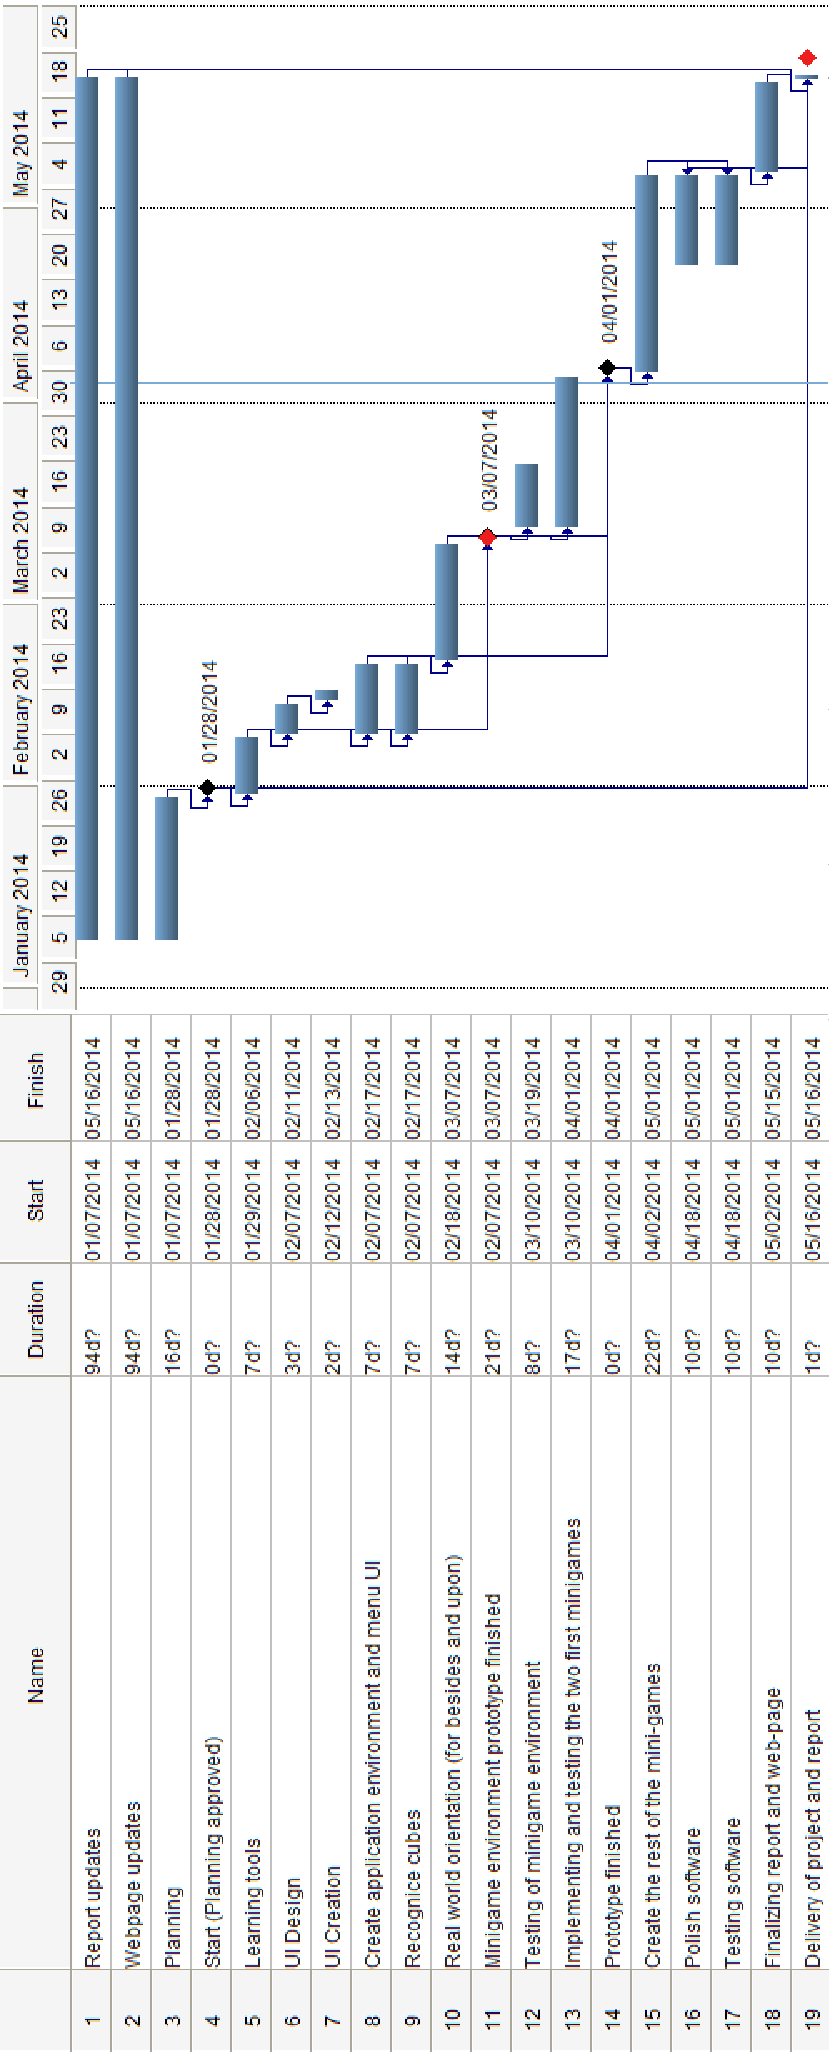
\includegraphics[height=\textwidth, angle=270]{preplan_gantt_diagram}
	\caption[Preplan Gantt diagram]{Our initial gantt diagram for the project.}	\label{fig:preplan_gantt}
\end{figure}


Afterwards we see that the process has been like this:

\todo{Insert gantt diagram of our dev-process here.}

\section{Planning vs reality}%Or how we worked compared to the plan
Our development cycle deviated a lot from the original plan due to a multitude of factors.
For instance we could have allocated less time to the "Create application enciromnet and menu UI" and "Recognice cubes" which each were allocated 7 days in the plan, but had we known more about Unity or the Vuforia plug-in in Unity then we would have known that Unity have methods and functions for creating in-game UI and to make the Vuforia plug-in working were just adding a \gls{prefab} for the camera.
We spent the time allocated to those time slots to creating the framework instead and this additional time shifted a lot of the sub-sequential work a week ahead of time.
Task number 10 (Real world orientation (for besides and upon)) was moved to the beginning of the project by developer Jakob and was done as part of him learning Unity.

The most drastic change in the time schedule is in item 11-15.
After learning some of the inner workings of Unity and how to properly set up a game in Unity it became rapidly apparent that we had taken a somewhat naive approach on it. This was due to our lack of knowledge of how much a game engine can do for us.
Using Unity we had a almost complete mini-game enviroment from the beginning. As such we only had to program what interaction we wanted to happen when cubes collided.
Our time and efforts were then spent on making the interaction between cubes and the player to what we wanted instead of having to focus on making the basics of a game world working.

		Here is a reference to chapter \ref{chap:project}. \comment{We can remove this}

		\section{Development process}
		\section{Development process}



	\chapter{Unity}
		\label{chap:Unity}
		\todo{Why...?}
\todo{Generally how it works. Generally how it does not work. Generally how it make people cry.}

Unity is a game engine and development enviroment.
It features a intergrated work enviroment with good tools that promotes rapid workflows to create the games you wish to create without worrying about the underlying structure.
With its multiplatform deployment tools and intergrated asset store it has become very popular for games.
Supporting both 2D, 3D and animating makes so that you dont need other programs to create what you wish to create.

Getting into Unity for the first time is greatly aided by the many video tutorials that Unity has created, showing how to use the interface, basics of scripting and programming, how to add sound and much more.



	\chapter{UnityScript}
		\label{chap:UnityScript}
		In Unity a user can use several different languages to script their games. Boo, C\#, JavaScript and Shader (used for writing shaders).
While Boo and C\#  use the standard implementation and is easily referenced the JavaScript used in Unity is not.\cite{WikiScriptVSScript}

Unitys JavaScript is quite different in many ways from the more standardly used JavaScript that is based on ECMAScript\cite{ECMAscipt} which is a standardized scripting
language standardized by Ecma International.

Some of the major and notable differences between Unitys JavaScript (henceforth named UnityScript) and ECMASCripts JavaScript (henceforth refered to as JavaScript):

\begin{itemize}
	\item Classes.
	\item Different privacy.
	\item var as a keyword is required.
	\item Not JavaScript library compatible.
\end{itemize}

\section {Classes}
JavaScript have no concept of classes as it is a prototypical language, meaning it will have the properties that is assigned to it, but is not bound to them.
Properties can be added or deleted at will in runtime, this is true for both members of the object and functions. UnityScript is much more object oriented with strongly typed and defined classes that cannot be changed in runtime (the exception to this rule is reflection).
This makes it difficult to work with UnityScript if you have little experience using it, or have yet to find out that the difference between JavaScriptand UnityScript.
UnityScript have also removed the prototypical properties of JavaScript by implementing it as a class based language. Meaning objects can not get additional functionality or be completely redifined at runtime. In UnityScript each .js file is implemented as a class by default. So when a developer creates a new .js file the Unity compiler and serialization system will add a class definition around the data within the file by default, so to call a funciton within a .js file you write "filename".function.

\section {Different privacy}
UnityScript, being structured like other object oriented languages have the usual levels of privacy of members within a class being markedas either Private, Protected or Public. JavaScript have per function privacy. Meaning a variable declared in a function is available in the entire function but not outside of the function.

\section {var as a keyword is required}
If you do not use the keyword var in JavaScript the variable becomes a global variable as the var keyword is used to denote scoping. In UnityScript the var keyword is required when creating a variable to make sure the scoping is always the intended scope.

\section {Not JavaScript library compatible}
UnityScript being so different from JavaScript makes other pre-made JavaScript library non-compatible with UnityScript, which also makes it really difficult to find reference help. One half of the built in library in Unitys Monodevelop is Unitys own library and the other half is made using what seems to be .NET framework from MicroSoft


	\chapter{Unity Serialization}
		\label{chap:UnitySerialization}
		Unity operates with two memory spaces. The native one belonging in to the C++ side of the code and the more managed DLL side that comes from scripts.
The managed side memory is where all the data from scripts that we as users are put.
To use the data Unity does something called assembly reload. What happens it that it pulls all the data out of the managed side, creates an
internal representation of the data on the C++ side, destroys all the memory from the managed side, reloads the assemblies and then
re-serialize the data from C++ into the managed side.
The serialization happens when the Editor or the system reloads an assembly, when the user enter and /or 
exits play mode and when the scene is loaded/ saved.
A serialization can therefore happen rather frequently or rarely, depending on the work-flow of the user
 and what the user is currently doing.
This is all well and good, until you get into one of the few corner cases where your data does not serialize into C++ and gets destroyed.

Unity is only able to serialize basic data types and those already defined within the MonoDevelop system that is part of Unity.
What this means is that if Unity does not know explicitly that the data are to be serialized or if it is unable
to serialize it, it will simply be destroyed. Most classes will not be serialized unless they have data that Unity 
can recognize is being used.
There are a few ways to make sure Unity knows that the data shall be preserved not destroyed:
\texttt{enumerate}
\begin{enumerate}
	\item Make the data field public
	\item Mark the field as serialize-able (@SerializeField in JavaScript and [SerlializeField] in C#)
	\item Mark the class as serialize-able (@Serialize in JavaScript and [Serialize] in C#)
	\item Make a class that derives its base type from ScriptableObject
\end {enumerate}

By having the data marked in either of those ways or a combination of them will ensure that Unity will try to
serialize it.
But there are a few things that Unity can not easily serialize, and most notably it can not serialize an array of normal objects.
It can serialize an array of objects that is derived from ScriptableObject. What the serialize will do is serialize each object in the
array individually and put a pointer into the array. To make this work the ScriptableObject derived class has to be in its own
C# file.
Unfortunately for us we are using the Unity engines JavaScript in this project, and getting C# and JavaScript to work nicely
together is not a trivial task in Unity.

The Unity serialization gave us as a group a lot of troubles, specifically with the data we wanted saved for each cube in scene.
For the cubes design we made a class named BoxDesign that was intended to contain all the data and functionality needed to 
control and set the design for the cubes in the game.
By following the guidelines from Unity on how to make the class serialize we made the class derive from ScriptableObject
and marked all non-public fields with @SerializeField and marked the entire class with @Serialize, but no matter what
 we tried to do the array we put the data into did not survive the assembly reload.
 It took most of the group the better part of three weeks of work and research on the matter to find a solution.
 After an enormously amount of attempts and fixes we ended up with a solution that while maybe not the best is reliable
  and functional. The solution was to encode the design into JSON and store the resulting string since strings are
   supported by the Unity serialization.

	\chapter{Development changes and decisions}
		\label{chap:Developmentchangesanddecisions}
		Following is a list of decisions and changes we as a group made during the development of this project in chronological order.

\begin{enumerate}
	\item 09.jan: As many as possible mini games should be created in a dynamic way.
	\item 09.jan: Graphics for the system does not have to be more advanced than what is shown in the design document.
	\item 09.jan: The cubes need only to have basic collision between others to achieve the functionality we need for the games.
	\item 09.jan: Our focus should be on making as many games as possible within the framework and not on making  a few perfect ones.
	\item 24.jan: We decided to shift our focus to be more on the framework itself and not the games within the framework.
	\item 30.jan: Costas wants us to implement a variation of the mobile app Wooords to replace a few of the other mini games.
	\item 31.jan: We decide to look into the implementation of Wooords at a later date in the development as it is a interesting game and will enhance the finished app since it is not similar to the other mini games.
	\item 10.feb: The group, along with Costas have decided to drop the memory mini game and the path mini game described in the design document.
	\item 17.feb: In the design document it implies that the loading screens should have all time leader board and a high score for the player. This is not consistent with the rest of the design document nor with our planning document and it was decided to instead have a high score for the current player on the loading screen instead.
	\item 06.mar: The design of the boxes is set in the inspector during the making of the game in Unity, the design can therefore not be changed during runtime.
	\item 10.mar: We decided to look into detached / integrated use of a AR library.
	\item 18.mar: Pictures that will be used as textures on the cubes must be in a folder called "/Resources/BoxDesign/" to be able to properly load them since we are not able to extract the path of where a texture is stored on disc.
	\item 27.mar: The levels for mini games will be procedural generated unless you want to make a Wooords mini game, where the levels will be read from file since these levels can not be easily randomly generated.
	\item 29.apr: The restart button have been removed from the pause screen.
\end{enumerate}

\subsection{Framework instead of games}
In the beginning we wanted to make sure that we would be able to create all the games described in the design document, and after looking into how we should structure the programs and what scripts and the like could be shared between each of the mini games we realized that on the programming side of them there was little difference. We therefore decided upon focusing making a framework to work within instead of making each mini game special.

\subsection{Implementing a word game instead}
Shortly after beginning development and starting testing of the \gls{Frame Marker} we realized that the mini game \#5: Memory cubes as it was described in the design document was not implementable. Playing the game would make the player turn the cube upside down in the best case scenario or covering the frame marker and then turn the cube in the worst case. This caused us a lot of problems because of the way that Vuforia controls its frame markers. What Vuforia does when it is not tracking a frame marker or it loses the tracking is to deactivate the frame marker in the scene hierarchy which makes us unable to access any information contained within both the frame marker object itself and its children. This meant that we had no reliable way to detect if the player turned a cube to see the hidden mark under the cube or if it was simply re-detected by the tracker due either by the player obscuring the marker or something else obscuring the marker or the marker just being lost for a few frames. We brought this issue to our employer and after a short discussion we came to the conclusion to implement our own version of the mobile game Wooords and not make the mini game \#5: Memory cubes and also to not make mini game \#6: Path as the game was deemed % nu nu nu
Woords is a game where the player is presented with a jumble of words and a theme. The goal is to find as many or all the words in the level by combining the letters to make words.


\subsection{Dropping leader-board}
In the original design document we got there was mention of having the loading screen both instructions for the game and a global leader-board. Unity does not work well with net based activities 

\subsection{Putting textures in a special folder}
This decision is due to a limitation in Unity. When you place a object in the object field in the inspector it will give us a new instance of that object, in this case a texture. What it does not give us is where it is stored. This would not be a problem if Unity was able to serialize our data, but since we are storing our objects as a JSON object due to Unity not being able to serialize it we have to store it ourself and the name of the texture is the only data we can rely on. The name however does not include the path of where the object is stored, so when we are extracting the data back from JSON objects into textures we only have the name of the texture. So to avoid any confusion of duplicate names and avoiding searching for the texture we constrict the location of where it can be placed into a sub-folder in the Resources folder of Unity.

\subsection{Procedural generation over predetermined levels}
In the beginning of the development we were uncertain about whether we should create levels for the mini games with code or if it should be crafted by hand. We initially went for the possibility of both, however after discussing it with our employer we came to the conclusion that as many of the games as possible should have generated levels. The only mini game that is not suitable for random generation is mini game \#7: Wooord game, the Wooord game has a single file for each set up starting with the overall theme (example is: animal, this means that all the words are animal related), followed by a comma separated sequence of what words should be on the cubes and on the line under is a comma separated list of words that can be created with those words. To create more levels the file just have to continue with a new sequence of letters for the cubes to have and a new line of words that can be created.

\subsection{The restart button has been removed from the pause screen}
\todo{Jakob kan skrive om hvorfor den f\o{}rst \o dela alt, men at vi senere fikset den.}

\part{Tools}

	\chapter{MonoDevelop}
		\label{chap:MonoDevelop}
		MonoDevelop is the integrated development environment (IDE) that comes with Unity. It supports writing in C\#, Unity JavaScript and Boo.
MonoDevelop is developed by Xamarin \cite{xamarinRef} as an open source integrated development environment for Windows, Linux and OS X.
Its primary focus is on C\# and other .NET languages.


MonoDevelop offers debugging features such as breakpoint, stepping trough code one line at a time, tracking of variables, call stack of functions and more.
It also have features to help with programming such as code completion and solution overview. Alongside all this it also supports add-in's for adding support for other languages.


\begin{wrapfigure}{l}{0.3\textwidth}
	\capstart
	\centering
	\vspace{-10pt}
	
\includegraphics[width=0.28\textwidth]{images/MonoDevelopLogo.png}
	\vspace{-20pt}
	\caption[MonoDevelop IDE Logo]{{M}ono{D}evelop {IDE}}
	\label{fig:monodevelop}
	\vspace{-10px}
\end{wrapfigure}

For us MonoDevelop gave mixed results. 
I have no doubt that it is a good IDE for working with C\# or a .NET language, but the UnityScript integration is poorly done.
The auto complete functions was flimsy at the best of times, most of the time it never activated and when it did it did not give the correct results. 
There has also been times when trying to get a public variable have resulted in a error because the variable has yet to be defined while it is available two lines above with no change in the scope.
We believe these problems are more due to Unitys implementation of JavaScript and not a error on MonoDevelops part, so if one are to use MonoDevelop we would recomend to shy away from Unitys JavaScript and use C\# instead.
Ending with on a positive note it had the best "Watch" feature we have come accros, it made tracking of several variables at a time really simple even if that variable was part of another script or class.	

\todo{Does this need more?}


	\chapter{Version Control}
		\label{chap:VersionControl}
		We have been using GIT for version control in this project. This is a version
control system we had some prior experience with, so we wanted to try it for 
this project as well. 

GIT works best with plain text files. With Unity there is quite many binary
files as well. At first we were not entirely sure how much of the files that
were binary and if GIT could work for us. After some googling we found that 
this was possible. On Unity's webpage they instruct on how to use the version
control system called Subversion \cite{SubversionControl}. Together with some
help from stackoverflow.com\cite{gitVersionControl} we figured out how to set 
up the project with GIT.

Unity produces .meta-files for each file in the project. We do not know 
entirely how these works, so we met some problems that we suspected had its
origin in these files. Because of this we have tried both to have them in
the GIT repository and not. The solution to that specific problem was not
clear when we got it working, so we do not know whether the metafiles were
problematic or not. The post at stackoverflow explained that the .meta-files 
could be set to hidden. This implies that the files should not be part
of the GIT repository. Anyway, now thay are because it seemed to help with the
problem we had, and it has not given any other problems later.


\begin{wrapfigure}{l}{0.3\textwidth}
	\capstart
	\centering
	\vspace{-10pt}
	
\includegraphics[width=0.28\textwidth]{images/git}
	\vspace{-5pt}
	\caption[GIT logo]{GIT}
	\label{fig:git}
	\vspace{-10pt}
\end{wrapfigure}

Many of the pure binary files has not been necessary to upload. Those that
has, like images, has often been of a type that didn't need to be updated
often. This means that most of the content in the repository could be plain
text and therefore we have been able to use GIT without further hassle.

\begin{wrapfigure}{r}{0.3\textwidth}
	\capstart
	\centering
	\vspace{-10pt}
	
\includegraphics[width=0.28\textwidth]{images/github}
	\vspace{-5pt}
	\caption[{G}it{H}ub logo]{{G}it{H}ub}
	\label{fig:github}
	\vspace{-10pt}
\end{wrapfigure}

We have used GitHub \cite{GitHub} as our online repository server. By using
this service we could easily share the work we have done. That we could use
an external server like this has been important for us when choosing version
control tool. Especially in one occation this proved to be very smart. One of
us encountered a bug in Unity that were quite severe. The Unity3D program
crashed, and by some unknown reason, it deleted a lot of files. The files that
were removed were all of the project files + some other files in the parent
directory. Many totally unrelated files were deleted and 4 days work that was
not committed to the server were lost. But fortunately enough, he could
download the lastest version from GitHub and use the last days lessons to write
the lost changes a whole lot faster.

When we have been using GIT we have used the commandline tool and also the GUI
program for GIT called Sourcetree \cite{SourceTree}.

The workflow we have been using has been very simplistic. We are aware that
there are good workflows that we could have used, but we have choosen to only
have a master branch that everyone pushes to. During the project we were told
about a way that worked for another group were they used pull requests and in
this way added an extra layer of security of code integrity. We tried this out
for a short time, but since none of us had experience with this way of working,
we discared it after a relatively short time. We were working quite close with
many small and rapid changes that we shared with everyone. If another group
member should accept this every time, we think that a lot of unnecessary time
could have been wasted on this. The model is not bad, but we have come to the
conclusion that it didn't fit our way of working very well. If we had started 
to do it from the beginning, we could maybe have done it, but the effort may
still have not been worth it. Anyhow, we are glad to learn about other ways of
working that can be useful later.

\part{Summary}

	\chapter{Afterword}
		\label{chap:afterword}
		\input{includes/cogARC_afterword}


\todo{Remove this when people know how to use glossaries or before delivery}
Here is an example on how to use glossaries. We can for example use the word
\gls{ECMAScript}. Now we get the text ECMAScript with a link to the glossary
list. In the glossary list there will also be a link to where this is 
referenced in the document. The same applies for \gls{serialization}.



% References
\bibliographystyle{classes/gucthesis}
\bibliography{includes/cogARC_bibliography}

% Glossary list
\printnoidxglossary[sort=word]


\part{Appendices}

\appendix %after this line all chapters will have leters instead of numbers
%\appendixpage
%\addappheadtotoc

% Examples
\chapter{Packages}
\label{chap:packages}

The \texttt{gucthesis} is built upon the standard \LaTeX\
\texttt{report} class. All commands from the \texttt{report} class can
be used, with the two exceptions of \verb+\subsubsection+ and
\verb+\paragraph+. This is because there should only be three
levels of headings according to the guidelines~\cite{GUCMaster}.

\section{Packages Used by gucthesis}
\label{sec:packages}

In addition to the \texttt{report} document class,
\texttt{gucthesis} makes direct use of the following packages
that must hence be present:
\begin{description}
	\item[geometry:] used for setting the sizes of the margins and
  	headers.
	\item[fontenc:] used with option \texttt{T1} for forcing the Cork font
  	encoding (necessary for the Charter font).
	\item[charter:] load Charter as the default font.
	\item[euler:] load the Euler math fonts.
	\item[babel:] to load language specific strings. Reasonable options
	  include \texttt{british}, \texttt{american}, \texttt{norsk},
	  \texttt{nynorsk} and \texttt{samin}.
\end{description}

\section{Other Relevant Packages}
\label{sec:otherpackages}

The author of a thesis might want to use a bunch of different packages
to those described in Section~\ref{sec:packages} in order to have all features needed for their document. 
In particular, it is advised to use the following:
\begin{description}
	\item[inputenc:] to allow \LaTeX\ to use more than 7-bit ASCII for its
	  input. Most often, the option \texttt{latin1} will do.
	\item[graphicx:] to include graphics.
	\item[hyperref:] this is a very nice package that makes cross links in
	  pdf documents. Use with option \texttt{dvips} or \texttt{pdftex}
	  in accordance with the driver that you use. Unfortunately, hyperref
	  is not completely bugfree\dots
\end{description}

\chapter{Structural Elements}
\label{chap:structural}

The title of the thesis should be set using the \verb+\thesistitle+
command, and the date of the thesis should be set using the
\verb+\thesisdate+ command. This makes the title and date appear in
the running header, like in this document.

\section{Page Layout}

The geometry of the page has been set using the \verb+\geometry+
command.

\section{Fonts}

Due to limited \LaTeX\ support for the Georgia font, Charter has been
chosen instead. For mathematical formula, the Euler fonts are used,
since they blend more nicely with the Charter than the standard
\LaTeX\ fonts: 
$$
 f(x) = \int_0^x g(\tau)\,d\tau
$$

For inline math you can use $\backslash{}($ and $\backslash{})$ for example \( f(x)= \frac{x^2}{1+x^2} \).  
This also allows you to use $\slash$ and $\backslash$. You need to include the \{\} when you want the special
character to have other letters immediately after it.

\section{Sectioning Commands}

The standard \LaTeX\ sectioning commands are used for both numbered
and unnumbered sections. The top level is given by the \verb+\chapter+
command. This starts a new right page. The two lower levels are
obtained using the \verb+\section+ and \verb+\subsection+ commands.
The standard \LaTeX\ \verb+\subsubsection+ and \verb+\paragraph+
commands have been disabled since their use is not encouraged by the
thesis guidelines. When you use these they will not be given numbers.  
They still appear in the document with highlighting but not in the 
table of contents.

\subsection{The subsection}

This is an example of a subsection.

\subsubsection{The subsubsection}

This is an example of a subsubsection.

\paragraph{The paragraph}

This is an example of a paragraph with a heading.

\section{Floats (Figures and Tables)}
\label{sec:floats}

Figures are placed in the \texttt{figure} environment. An example is
shown in Figure~\ref{fig:example}. %notice the ~ in between figure and the \ref. it stops latex from splitting the number and word over a line.
Tables are placed in the \texttt{table} environment. An example is given in
Table~\ref{tab:example}. Figures and tables float freely around in the
document in accordance with standard \LaTeX\ behavior.

\begin{figure}[tbp]  %t top, b bottom, p page | you can also use h to try to get the figure to appear at the current location
  \centering
  
\includegraphics[width=.5\textwidth]{example_fig}
  \caption[An example figure.]{An example figure. If the caption is
    shorter than one line, it is centered. If it goes over more than
    one line, it is left and right justified. Furthermore, it is
    suggested that an alternative short caption is given in order to
    produce a good list of figures.}
  \label{fig:example}
\end{figure}

\begin{table}[tbp]
  \centering
  \begin{tabular}{c|c}
    Age  & IQ  \\ 
    \hline
    10   & 100 \\
    20   & 100 \\
    30   & 150 \\
    40   & 100 \\
    50   & 100
  \end{tabular}
  \caption{An example table.}
  \label{tab:example}
\end{table}

The captions are placed \emph{below} both for the figures and the
tables. The caption is set in 9pt. If the caption is shorter than one
line, it is centered.

\section{Quotes}
\label{sec:Quotes} % this allows you to refer to this section number using \ref{sec:Quotes}

Quotes are inserted using the standard \LaTeX\ \texttt{quote}
environment. The environment has been changed so that a 9pt font is
used:

\begin{quote}
  ``And I looked, and, behold, a whirlwind came out of the north, a
  great cloud, and a fire infolding itself, and a brightness was about
  it, and out of the midst thereof as the colour of amber, out of the
  midst of the fire. Also out of the midst thereof came the likeness
  of four living creatures.''
\end{quote}

\section{Lists}
\label{sec:lists}

Point lists and enumerated lists are made by using the standard
\texttt{itemize} and \texttt{enumerate} environments, respectively.
The spacing is going to be changed in accordance with the specification. For
\texttt{itemize}, the results look like this:
\begin{itemize}
	\item First item.
	\item Second item. Here I will put some long text, just to illustrate.
	  Here I will put some long text, just to illustrate. Here I will put
	  some long text, just to illustrate. Here I will put some long text,
	  just to illustrate.
	\item Third item also has subitems:
	  \begin{itemize}
		  \item First subitem.
		  \item Second subitem.
		  \item Third subitem.
	  \end{itemize}
\end{itemize}
and for \texttt{enumerate} like this:
\begin{enumerate}
	\item First item.
	\item Second item. Here I will put some long text, just to illustrate.
	  Here I will put some long text, just to illustrate. Here I will put
	  some long text, just to illustrate. Here I will put some long text,
	  just to illustrate.
	\item Third item also has subitems:
	  \begin{enumerate}
		  \item First subitem.
		  \item Second subitem.
		  \item Third subitem.
	  \end{enumerate}
\end{enumerate}

You may also want to use descriptive lists
\begin{description}
	\item[First] the first item.
	\item[Second] the second item. Here I will put some long text, just to illustrate.
	  Here I will put some long text, just to illustrate. Here I will put
	  some long text, just to illustrate. Here I will put some long text,
	  just to illustrate.
	\item [What now] the third item also has subitems:
	  \begin{enumerate}
		  \item First subitem.
		  \item Second subitem.
		  \item Third subitem.
	  \end{enumerate}
\end{description}


\section{Bibliographic References}

You should cite articles~\cite{Askvall1985}, books~\cite{Card1983},
anthologies~\cite{Lancaster1985} and web publications~\cite{Meldon1997}
like this. There is always an issue referencing web pages. Currently
we suggest that you use the HiG Website~\cite{HiG:Website}.


A particular bibliography style file for GUC named
\texttt{gucthesis.bst} has been developed based upon the
standard Bib\TeX\ \texttt{unsrt} style.


\chapter{Meetings}

You can include an Appendix of the log of your meeting for example

\GUC, 
\comment{so what}

\todo{task \#1}
This is a todo-task we need to get done.

\end{document}